\frame{
  \frametitle{Objetivos}

Debemos definir unos objetivos: generales, realistas y teniendo en cuenta el
contexto.

\begin{figure}[htb]
\centering
	
\includegraphics[width=4cm]{images/target}
\caption{Objetivos.}
\end{figure}

}

\frame{
  \frametitle{Objetivos}

\begin{exampleblock}{Lista de Objetivos}
\begin{enumerate}[<+->]
\item Estudiar y aplicar la semántica para formalizar modelos de conocimiento
compartido de un sector de negocio. 
 \item Estudiar el uso de modelos de conocimiento compartido para unificar
modelos de datos divergentes en un mismo sector de negocio.
 \item Proponer y definir una arquitectura SOA utilizando un modelo de
conocimiento compartido de un sector de negocio unificando modelos
de datos y operaciones. 
 \item Validar de la propuesta realizada. 
\end{enumerate}
\end{exampleblock}

}

\frame{
  \frametitle{Objetivos}

\begin{exampleblock}{Teniendo en cuenta:}
\begin{enumerate}[<+->]
\item El uso de estándares.
\item La delegación en productos ya existentes y probados.
\item El estado del arte de la tecnología.
\item Las sinergias con otros proyectos.
\end{enumerate}
\end{exampleblock}

}


\frame{
  \frametitle{Objetivos}

Porque no estamos solos~(``Trends the Internet of
Services''~\footnote{\url{http://cordis.europa.eu/fp7/ict/ssai/home\_en.html}}).

\begin{figure}[htb]
\centering
	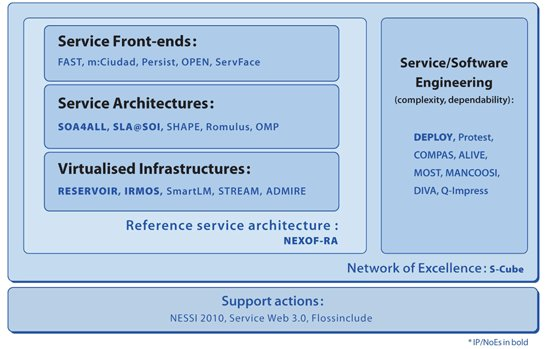
\includegraphics[width=6cm]{images/fp-projects}
\caption{Tendencia en Proyectos Europeos-FP7.}
\end{figure}



}